\documentclass[]{report}
\usepackage[francais]{babel}
\usepackage[utf8]{inputenc}
\usepackage{graphicx} %'affichage des images

\title{Rapport projet conception logicielle}
\author{Romuald GAFFE\and Yanis COSNEFROY\and Vy Vu NGUYEN PHUONG\and Alexandre BOURGOIN}
\date{\today}


\begin{document}
\maketitle 
\tableofcontents
\part{Objectifs du projet}
\section{Présentation du concept}
Tout d'abord, nous avons choisis de créer un puzzle block. Nous voulions que ce jeu soit simple d'utilisation afin que tout le monde puissent y jouer. Le block puzzle se présente sous forme d'une grille avec 3 figures que l'on appelle des objets que l'on doit placer dans la grille. Les objets apparaissent aléatoirement et doivent tous être placés dans la grille.Si la grille est complète, alors une apparition d'un GameOver va s'afficher en montrant le score de la personne. Sur cette page, le joueur aura la possibilité de retourner au menu ou de recommencer. Ensuite, dans le menu du jeu conçu, nous avons décidé d'y mettre 3 cases affichant le mode solo, le mode multijoueur et quitter le jeu. Si je le joueur clique sur le solo, alors le jeu va se lancer automatiquement. Si le joueur veut jouer en multijoueur, alors 3 autres possibilités vont être proposées. Ces 3 possibilités sont de jouer contre une intelligence artificielle, jouer avec une autre personne sur le même écran que l'on a nommé jouer en local et enfin jouer en ligne. Si l'on joue par exemple contre l'intelligence artificielle, alors il n'y aura pas l'apparition de sa grille pour éviter de la triche. Cependant, si le joueur décide de joueur en local, alors les 2 joueurs devront jouer une fois sur 2 car leurs grilles apparaissent une fois sur deux. Pour le mode multijoueur, À REMPLIR DÈS QUE LE MULTI SERA FAIT!!!!!! Des photos montrant des extraits du jeu seront présentés dans les exemples du jeux publiés

\section{Cahier des charges}


\section{Exemples du jeux publiés}
Voici plusieurs block-puzzle provenant de jeux.fr, et des applications pour android: \\
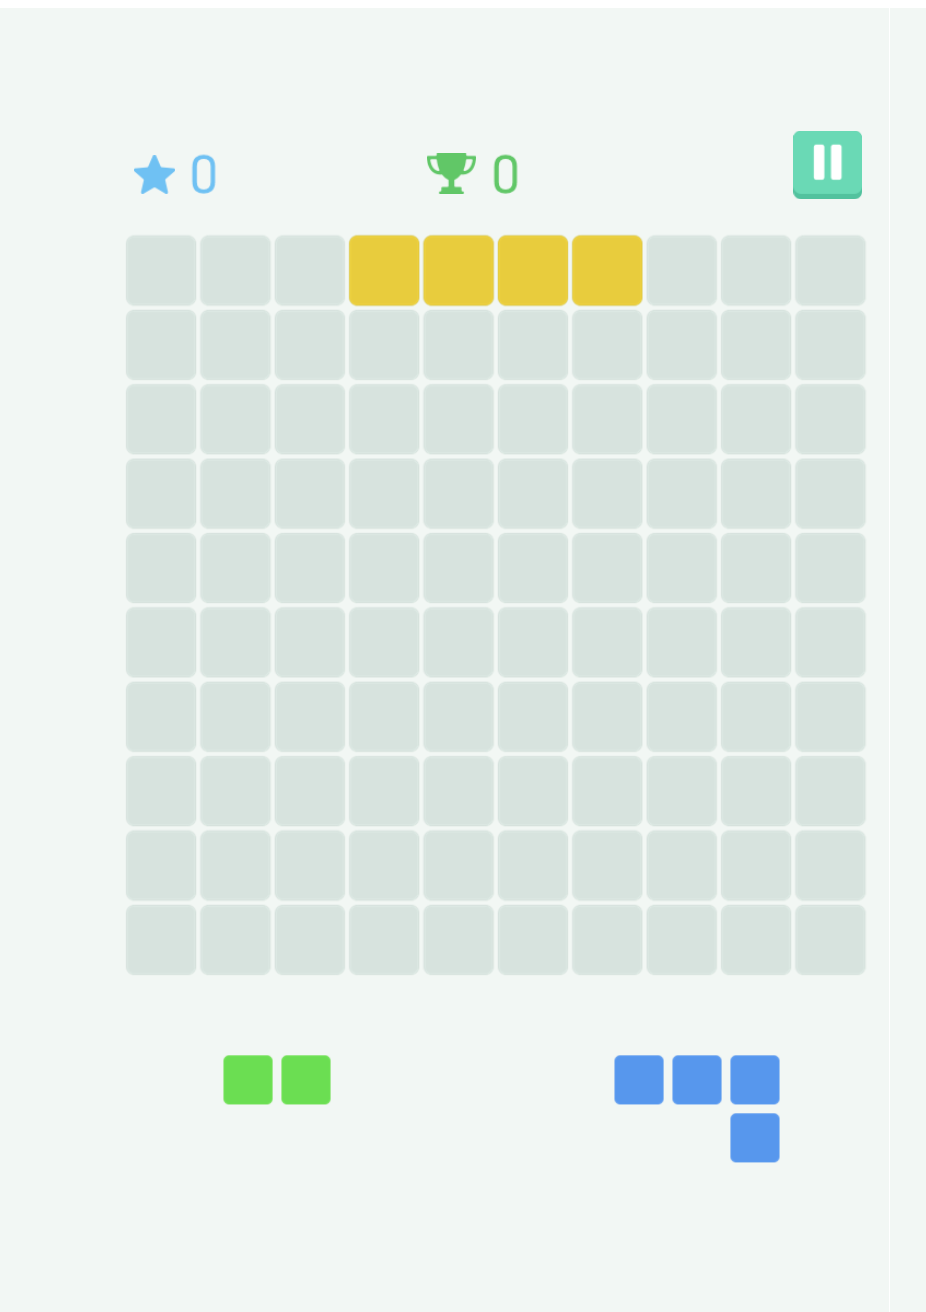
\includegraphics[scale=0.3]{images/jeuxPublie1.png}
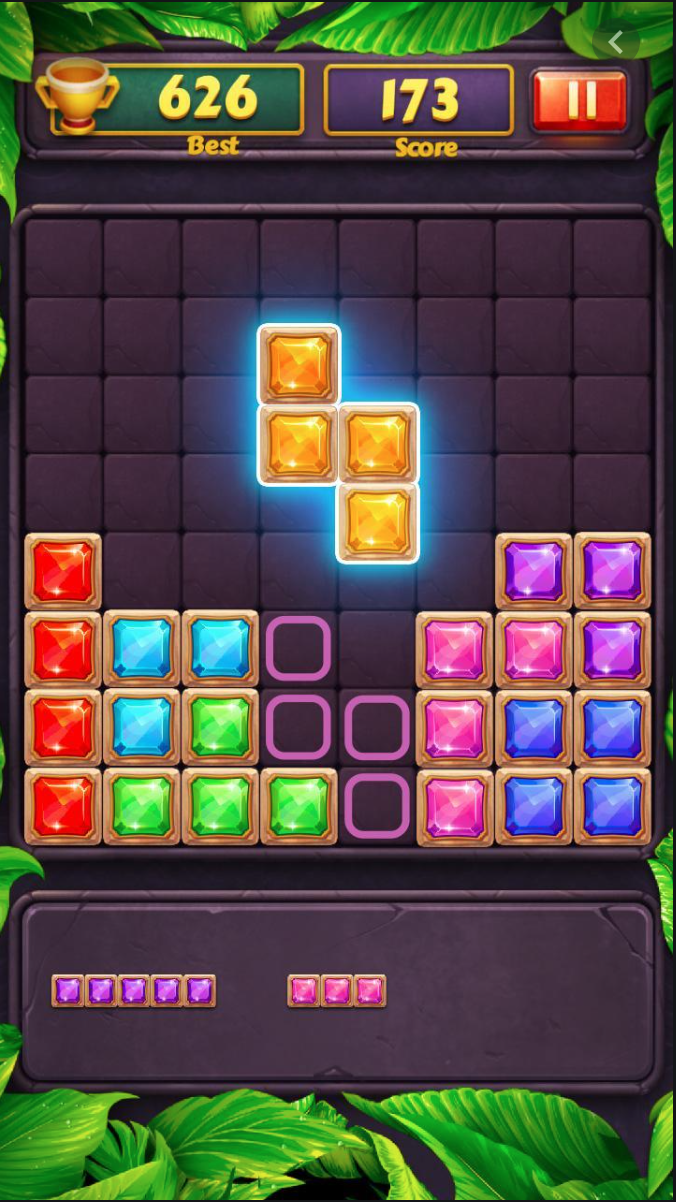
\includegraphics[scale=0.3]{images/jeuxPublie2.png}
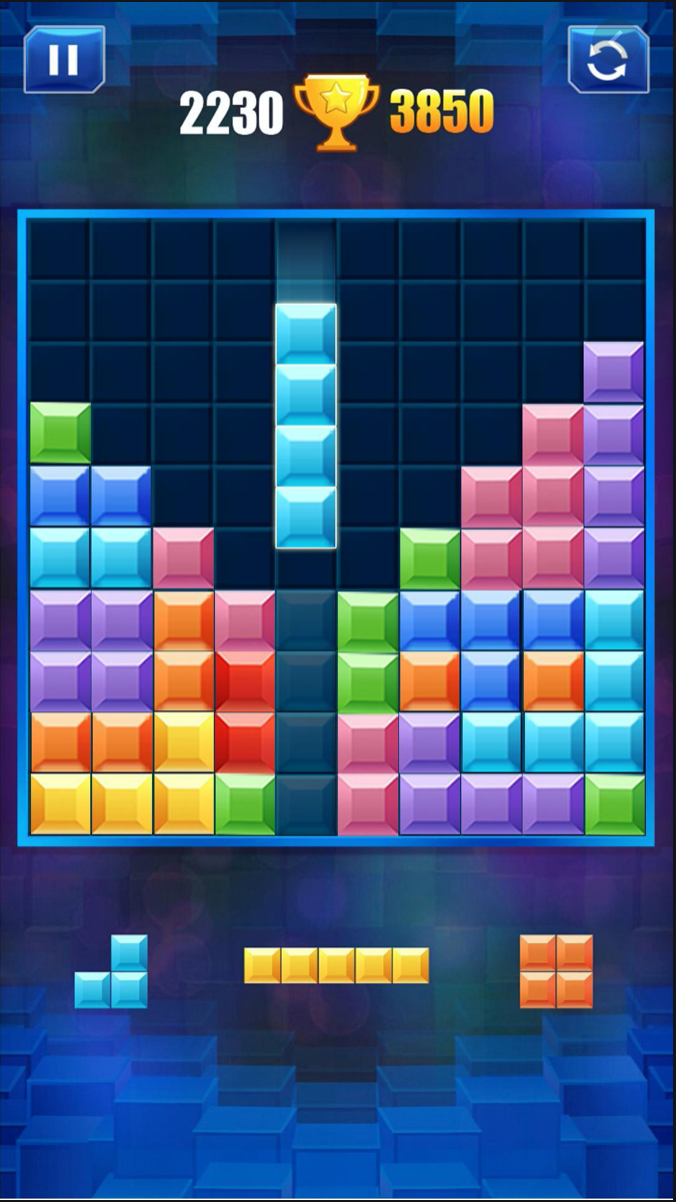
\includegraphics[scale=0.3]{images/jeuxPublie3.png}\\

On peut y retrouver les mêmes caractéristiques que notre projet. Notre projet a été conçu sur une base classique de block-puzzle qui réunit ces trois images montrées précédemment. Les différences entres ces block-puzzles et le notre sont la décoration du jeu ainsi que la sauvegarde du meilleur score établis sur le jeu par le joueur. On peut constater à l'essai de notre block-puzzle uniquement l'apparition des scores qui vont être actifs en fonction du jeu du joueur. Cependant nos règles sont un peu différentes par rapport au jeu déjà publié. On a décidé de ne pas rajouter de bonus ou d'aide à chaque fois qu'une ligne ou une colonne est remplie. C'est un choix volontaire pour provoquer une augmentation de concurrence de jeu avec d'autres joueurs mais aussi pour une adaptation plus développée de la difficulté de jeu. 
\part{Fonctionnalités implémentés}
\section{Mode solo}
\section{Mode multijoueur}
\subsection{Joueur vs Intelligence artificielle}
\subsection{Joueur vs Joueur en local}
\subsection{Joueur vs Joueur en ligne}

\part{Éléments techniques}
\section{La grille}
\section{Les pièces}
\section{L'aléatoire}
\section{L'intelligence artificielle}
\section{Le réseau}

\part{Architecture du projet}
\section{Diagrammes des modules et des classes}
\section{Cas d'utilisation}

\part{Conclusion}


\end{document}
